%%
%% This is file `sample-xelatex.tex',
%% generated with the docstrip utility.
%%
%% The original source files were:
%%
%% samples.dtx  (with options: `sigconf')
%% 
%% IMPORTANT NOTICE:
%% 
%% For the copyright see the source file.
%% 
%% Any modified versions of this file must be renamed
%% with new filenames distinct from sample-xelatex.tex.
%% 
%% For distribution of the original source see the terms
%% for copying and modification in the file samples.dtx.
%% 
%% This generated file may be distributed as long as the
%% original source files, as listed above, are part of the
%% same distribution. (The sources need not necessarily be
%% in the same archive or directory.)
%%
%% The first command in your LaTeX source must be the \documentclass command.
\documentclass[sigconf,nonacm]{acmart}

%%
%% \BibTeX command to typeset BibTeX logo in the docs
\AtBeginDocument{%
  \providecommand\BibTeX{{%
    \normalfont B\kern-0.5em{\scshape i\kern-0.25em b}\kern-0.8em\TeX}}}

%% Rights management information.  This information is sent to you
%% when you complete the rights form.  These commands have SAMPLE
%% values in them; it is your responsibility as an author to replace
%% the commands and values with those provided to you when you
%% complete the rights form.


%\setcopyright{acmcopyright}
%\copyrightyear{2019}
%\acmYear{2018}
%\acmDOI{10.1145/1122445.1122456}

%% These commands are for a PROCEEDINGS abstract or paper.
%\acmConference[Woodstock '18]{Woodstock '18: ACM Symposium on Neural
%  Gaze Detection}{June 03--05, 2018}{Woodstock, NY}
%\acmBooktitle{Woodstock '18: ACM Symposium on Neural Gaze Detection,
%  June 03--05, 2018, Woodstock, NY}
%\acmPrice{15.00}
%\acmISBN{978-1-4503-XXXX-X/18/06}


%%
%% Submission ID.
%% Use this when submitting an article to a sponsored event. You'll
%% receive a unique submission ID from the organizers
%% of the event, and this ID should be used as the parameter to this command.
%%\acmSubmissionID{123-A56-BU3}

%%
%% The majority of ACM publications use numbered citations and
%% references.  The command \citestyle{authoryear} switches to the
%% "author year" style.
%%
%% If you are preparing content for an event
%% sponsored by ACM SIGGRAPH, you must use the "author year" style of
%% citations and references.
%% Uncommenting
%% the next command will enable that style.
%%\citestyle{acmauthoryear}

%%
%% end of the preamble, start of the body of the document source.
\begin{document}

%%
%% The "title" command has an optional parameter,
%% allowing the author to define a "short title" to be used in page headers.
\title{Movie Search Engine Based on Description}

%%
%% The "author" command and its associated commands are used to define
%% the authors and their affiliations.
%% Of note is the shared affiliation of the first two authors, and the
%% "authornote" and "authornotemark" commands
%% used to denote shared contribution to the research.
\author{Dongjian Chen, Ren Wang, Yumeng Shao}
%\authornote{Both authors contributed equally to this research.}
\email{djichen@umich.edu}
\email{renw@umich.edu}
\email{emilysym@umich.edu}
\affiliation{%
  \institution{School of Information, University of Michigan}
  \city{Ann Arbor}
  \state{Michigan}
}



%%
%% By default, the full list of authors will be used in the page
%% headers. Often, this list is too long, and will overlap
%% other information printed in the page headers. This command allows
%% the author to define a more concise list
%% of authors' names for this purpose.
\renewcommand{\shortauthors}{Dongjian Chen, Ren Wang, Yumeng Shao}

%%
%% The abstract is a short summary of the work to be presented in the
%% article.
\begin{abstract}
  In this report, we describe our work on description-based movie retrieval. Our search engine is motivated by the idea of helping people retrieve movies when they could only remember fragments of the movies. We adopted a dataset with movie titles, descriptions and keywords as our search database. BM25+ function is adapted after we preprocess the dataset with with tokenizing, stemming, stopword and punctuation removal, and keyword addition. By calculating the harmonic mean of the ranks of the desired answers in our test cases, we are able to evaluate our system and conclude that our search engine has a fairly good performance.
\end{abstract}


%%
%% Keywords. The author(s) should pick words that accurately describe
%% the work being presented. Separate the keywords with commas.
\keywords{movie, BM25+, information retrieval, search}


%%
%% This command processes the author and affiliation and title
%% information and builds the first part of the formatted document.
\maketitle

\section{Introduction}

Watching movies has become one of the most popular ways of entertainment, and there are hundreds and thousands of new movies being released every year. The information we recieve is explosing and the challenge of remembering the right title for movie plots is becoming larger and larger, since an average person could have watched dozens or hundreds of movies. It is not rare for someone to bump into an annoying situation when they could only remember a rough story or some segments of the movie, but just could not recall its name. In such cases without a specialized movie search engine, existing search websites will return various results that include not only movies and the search results would not be very ideal with queries composed of common terms but has specialized meanings and indications when it comes to movies.

As a result, we we aim at helping people retrieve the film they want when they could only remember a part of the story plot or segments like character names and special props. The search engine we designed and implemented helps with finding the corresponding movies with description or keywords provided by the user that specialize in movies.

\section{Design Description}

The whole process of our design process including getting data, processing data, selecting model and building interface. And the working process of our final design is shown as following figure,

\begin{figure}[H]
  \centering
  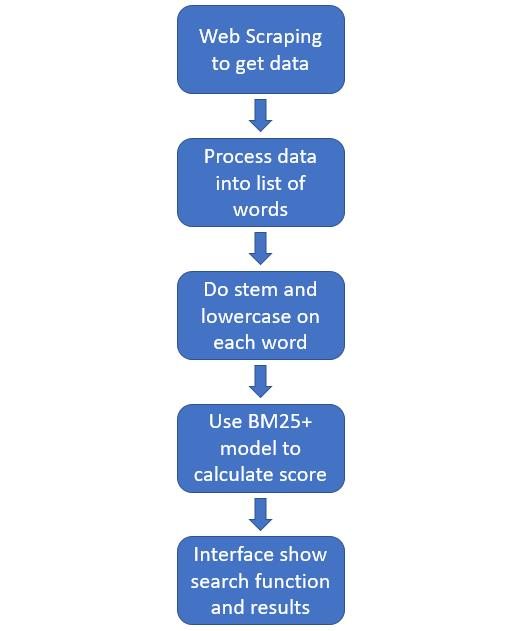
\includegraphics[width=0.5\linewidth]{process.jpg}
  \caption{Working process of our searching system}
\end{figure}

\subsection{Dataset}
We obtained our data from two sources:

Kaggle movie dataset:
\url{(https://www.kaggle.com/rounakbanik/the-movies-dataset#movies_metadata.csv)}

IMDB website
\url{(https://www.imdb.com/?ref_=nv_home)}

We first download a csv file from Kaggle with data about overviews and imdb link for each movie. We first try to use these overviews as documents for queries. Then we find that the performance of searching can't fulfill our satisfication so we try to find more documents. Finally, after tring the summary on wikipedia and total scene description on IMDB, we choose keywords on IMDB and use python webscraping to get these data.

\subsection{Basic Data processing}

In this project, our retrieval system is built to retrieve movie by its description and our data document for each movie contains its overview and keywords related to it.

We first scrape keyword data from a website and combined it with the overview of each movie from the Kaggle dataset into one string. Then, we tokenize the string into words and do stem and lowercase on each word and get lists of words for each document. Finally we remove stopwords and punctuations, and  the document is then ready for query. The above mentioned steps are also applied to query sentences.

\subsection{Advanced Data processing}

We tried two advanced methods on data to see if the performance of search can be enhanced.

First, we thought of adding the synonyms of each words in query so that those words with similar mean as query words in documents would not be missed. For each query we used nltk wordnet to get synonyms for each word in the query and added them into the query. However, the performance become worse instead of bettern. We thought that may be adding synouyms made the query vaguer so that more unrelated results are searched.

Also, we thought of adding weight to different kind of words in query. But that will led to another question that how should we judge the importance of different words. We thought of using part-of-speech tagger to tag each words in query and give more weight to adjectives and verbs. However, there is no distince improvement in the performance of our system. We can do further improvement on our system by trying to find more proper weighting methods on queries.

\subsection{Model}

We first use BM25 score function which is use to give score to each query-document pair by the term frequency(TF) of each word in the query and inverse document frequency (IDF) as following:

{
\Small
$$
  S = \sum_{t \in q} \cdot\left[\frac{\left(k_{1}+1\right) \\ \cdot c_{t}^{d}}{c_{t}^{d}+k_{1} \cdot\left(1-b+b \cdot \frac{l_{d}}{L}\right)}\right] \cdot \ln \left(\frac{N+1}{N_{t}}\right)
$$
}

However, the performance of BM25 score function is not so good so we want to find a more proper score function. We tried BM25+ function. The differences between BM25+ and BM25 are that BM25+ add an additional parameter and consider the frequency of each words in query. Since the performance of BM25+ is better and can relatively meet our needs, we finally choose it as our final score function (Inspiration from \url{https://www.eecis.udel.edu/~ypeilin/pub/ictir2016_long.pdf)} which is,

{
\Small
$$
  S = \sum_{t \in q} \frac{\left(k_{3}+1\right) \cdot c_{t}^{q}}{k_{3}+c_{t}^{q}} \cdot\left[\frac{\left(k_{1}+1\right) \\ \cdot c_{t}^{d}}{c_{t}^{d}+k_{1} \cdot\left(1-b+b \cdot \frac{l_{d}}{L}\right)}+\delta\right] \cdot \ln \left(\frac{N+1}{N_{t}}\right)
$$
}


This BM25+ function add two more parameters to change the weight of TF and IDF in the function and it make our performance better in our test query set. The performance comparison and analysis will be detailedly discussed in Result and evaluation part.

\subsection{Interface}

We have also built an interface for users to input the description they remember and will return the result movie name and simple overview. The movie with best score will be shown on the page and user can see more results with lower scores if he slide down the page as following graphs,


\begin{figure}[H]
  \centering
  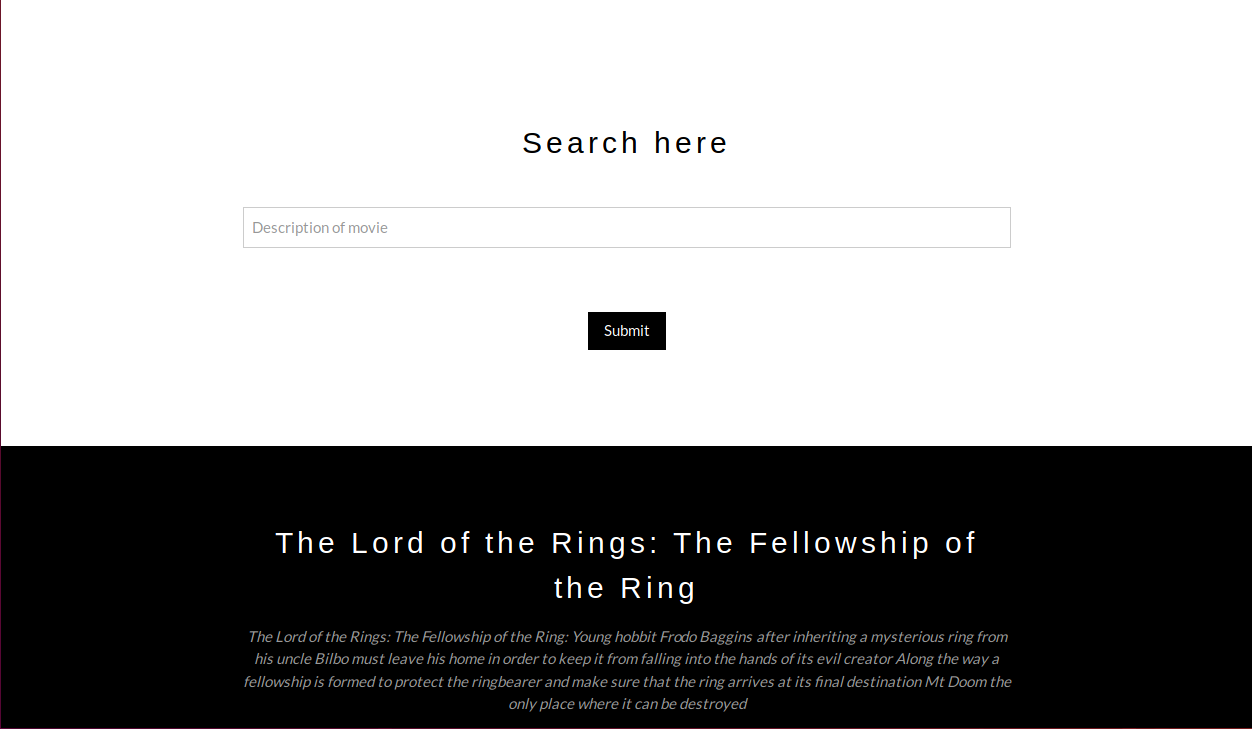
\includegraphics[width=0.8\linewidth]{interface.jpg}
  \caption{Interface}
\end{figure}

\begin{figure}[H]
  \centering
  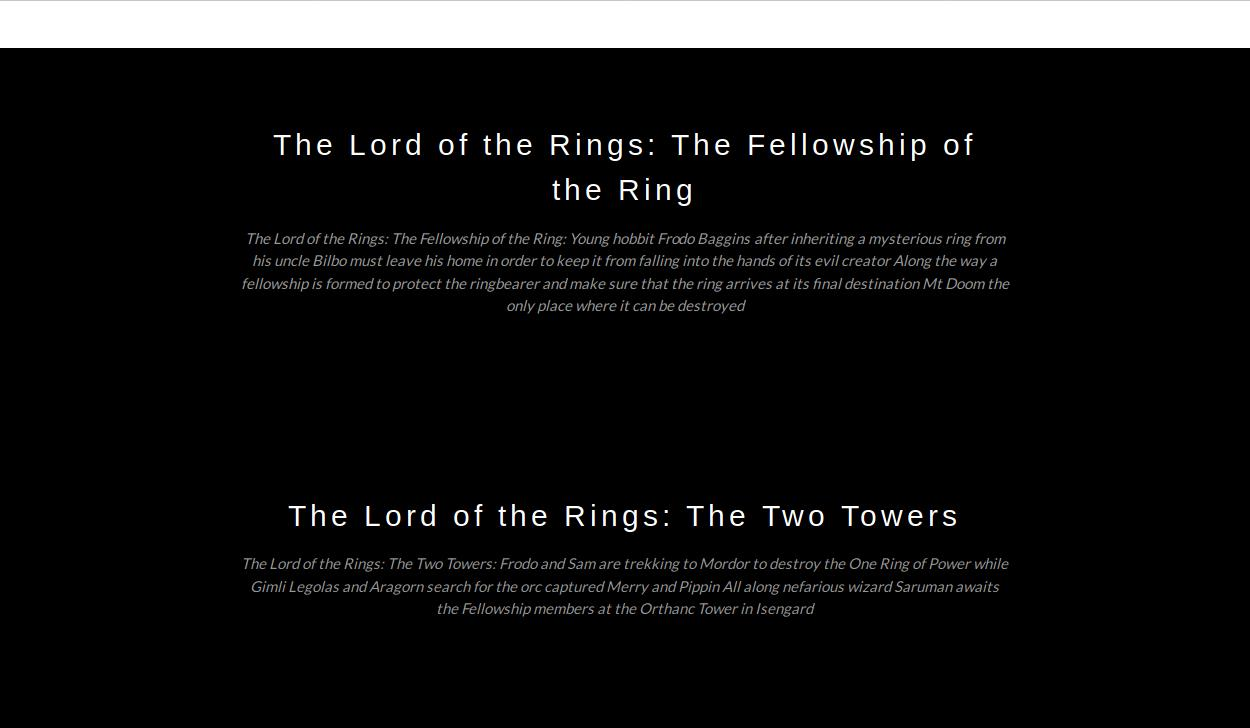
\includegraphics[width=0.8\linewidth]{interface1.jpg}
  \caption{Interface slide down}
\end{figure}

\section{Results and evaluation}

We formulate 35 short descriptions of movies and use our search engine to
fetch the result.
Some of the queries come from us and some of them are from our user during
the testing phase of our development.
For each description, we check if the intended result is returned by the
search engine.

Then we check the rank $R$ of the expected movie returned by the search
engine.
We define $\frac{1}{R}$ as the precision of our search engine.
We calculate the harmonic mean of $R$ (if the expected movie isn’t retrieved
within the first 10 movies, R is infinity.) and use it as the evaluation for
the search engine.

This is part of the testing result from our search engine, the third coloum
is the rank of the movie title retrieved based on BM25 BM25 and the fourth
coloum is for BM25+.


\begin{table}[H]
  \caption{Part of Our Queries Test Result}
  \label{tab:query_result}
  \begin{tabular}{llcc}
    \toprule
    Query             & Answer         & $\frac{R}{\text{BM25}}$ & $\frac{R}{\text{BM25+}}$ \\
    \midrule
    Jack and rose     & Titanic        & 2                       & 1                        \\
    Dinosaur          & Jurassic World & 4                       & 1                        \\
    France revolution & Les Misérables & 4                       & 2                        \\
    Dream thief       & Inception      & 6                       & 1                        \\
    Boy magic school  & Harry Potter   & 9                       & 1                        \\
    Cowboy astronaut  & Toy story      & 5                       & 1                        \\
    Robot kill human  & Terminator     & 4                       & 1                        \\
    \bottomrule
  \end{tabular}
\end{table}

The harmonic mean of rank of the expected movies can evaluate the average
results the user need to skim through to find the movie they intend to have.
Thus, the lower harmonic mean of rank, the better engine we have.
The following is the harmonic mean of rank result of BM25 and BM25+.


\begin{table}[H]
  \caption{Comparison of Harmonic Mean of Rank }
  \begin{tabular}{ c  c c}
    \toprule
                                              & BM25  & BM25+ \\
    \midrule
    $ n / \sum_{i=1}^{i=n} \frac{1}{R_{i}}  $ & 2.944 & 1.449 \\
    \bottomrule
  \end{tabular}
\end{table}

The following is the figure showing the sorted distribution of expected movie retrieved ranks.
For the figure for BM25, there are a lot of queries that returns failure (greater than 10),
while for BM25+, there is no failure and the mean of ranks is obviously lower.


\begin{figure}[H]
  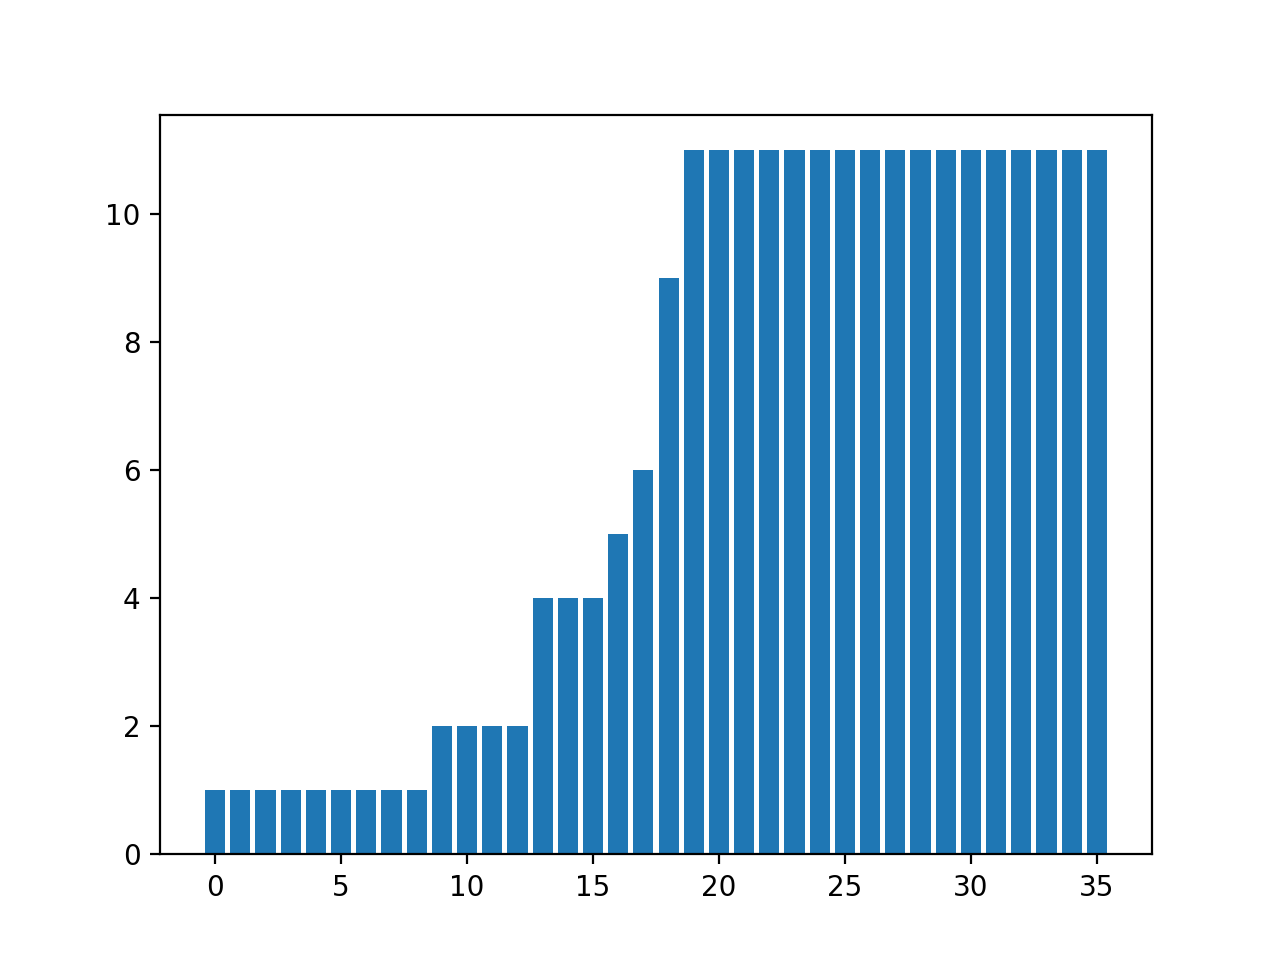
\includegraphics[width=0.47\linewidth]{evaluation_1.png}
  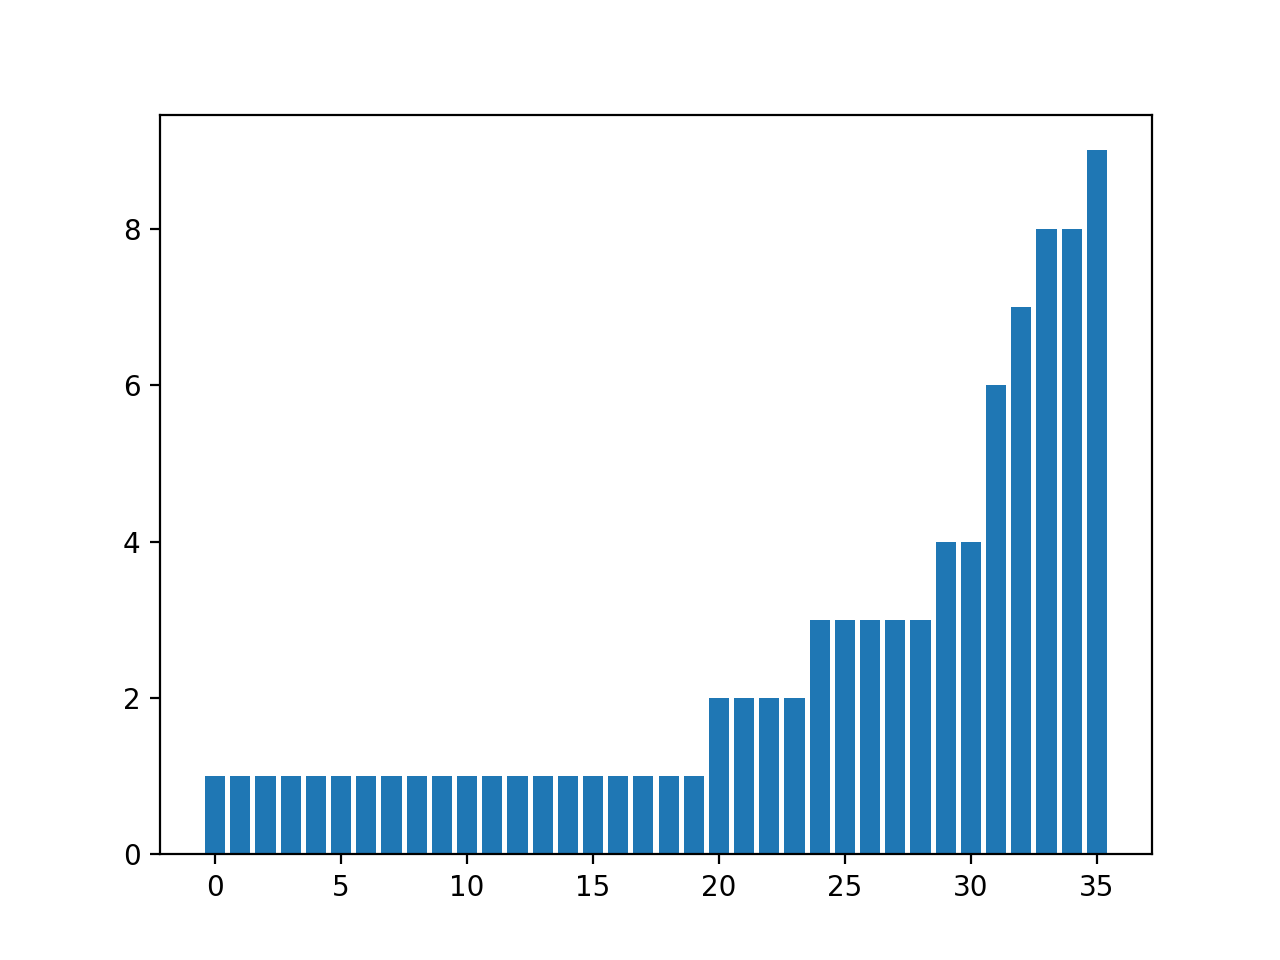
\includegraphics[width=0.47\linewidth]{evaluation_2.png}
  \caption{Expected Movie Retreived Ranks Distribution}
\end{figure}

Thus we can evaluate our search engine as useful, for on average the user
can expect to find the moive they want from the first and second result
retrieved.

\subsection{Comparison between our search engine and Google}

It's hard to quantatively compare our search engine's capability with
Google, because for each query, Google returns results of webpages, images
and even links to external websites.
However, the common behavior of Google is to treat the query ``as it is''.
For example, when the user wants to find the movie ``Jurassic World'' when he or she only remembers
scenes of Dinosaurs, Google will return some sophisticated documentary
movies of ``Dinosaur'', but what the user really want is ``a popular movie in
which dinosaurs show up''.
Thus, for accomplishing the job of searching movie based on fragments of description, our search engine
can beat Google.


\section{Conclusions}

The result of this project is generally satisfying with our experiments with
it. We succeeded in returning the related results with the queries and has
improved its performance with data processing and parameter tuning. Thus,
with our search engine, people can mostly get the movie they referred to.
However, the search engine might not work well with subjective feelings on
movies since the data we used for query are neutral descriptions.

\section{Future Improvements}
During data processing, we have tried part of speech tagging on the sentence and give more weights to certain types. However, it doesn’t turn out well as we expected. We believe that digging further into this by analyzing the parse tree to evaluate the part of speeches more precisely can help with giving better weights.
Moreover, we believe that keeping a search and view log can also help with improving accuracy. Within a series of similar searches, we can analyze the movies the user has clicked into and find the similarities to feed back into the algorithm and adjust the weights accordingly.

\begin{acks}
  Prof. Qiaozhu Mei, Mr. Wei Ai from University of Michigan;
  Teaching Assistant [Shiyan Yan, Xinyan Zhao] for SI 650 at University of Michigan.
\end{acks}


%% ============================================
%% ============================================
%% ============================================
%% ============================================


\bibliographystyle{ACM-Reference-Format} 
\bibliography{refs}


\end{document}
\endinput
%%
%% End of file `sample-xelatex.tex'.
